\section{Feature matching}

\subsection{Question 1}

{\bfseries Modify the previous threshold. What is the effect of this
threshold? Comment your response.}

We can see the result of the default matching process in figure \ref{fig:matching15thres}.

\begin{figure}[htb]
	\centering
		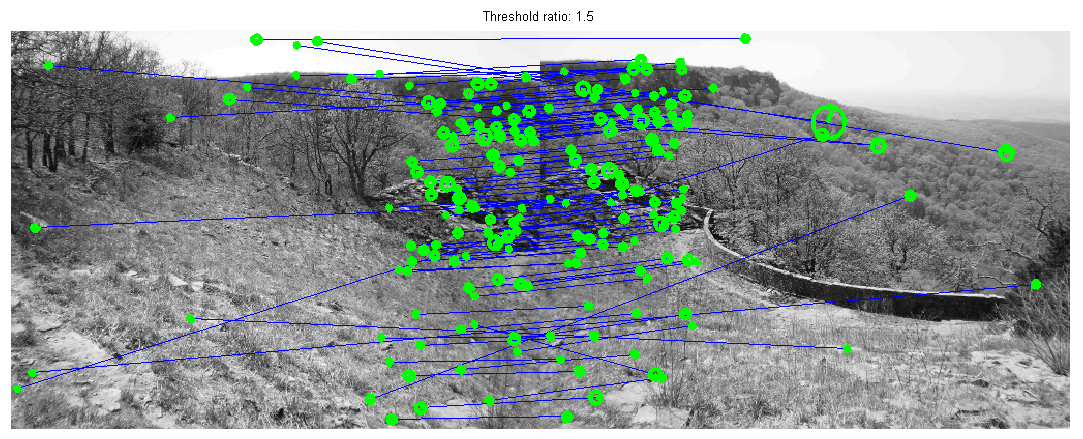
\includegraphics[width=\textwidth]{./img/ex1/matching_15_thres.png}
	\caption{Result of matching with a threshold ratio of 1.5 (default)}
	\label{fig:matching15thres}
\end{figure}

We have also computed the matches using different thresholds. In figure
\ref{fig:matching20thres} we can see the result of the matching algorithm
with a threshold ratio of 2.0. It is clear that there are fewer matches. This is
due to the fact that the ratio between the distances to the first and second best
matches acts as an uniqueness measure. Therefore increasing the threshold leads
to a more restrictive selection of the relevant matches and to a lower number of
matches at the end.

\begin{figure}[htb]
	\centering
		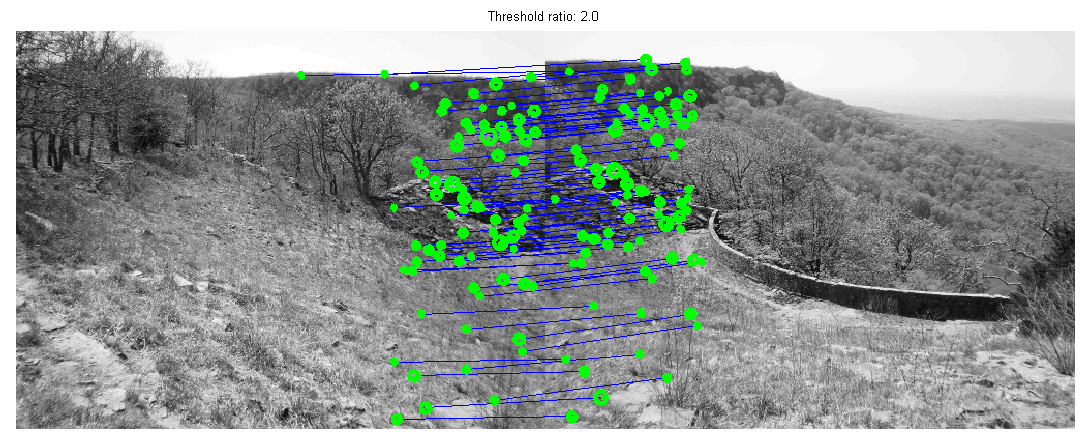
\includegraphics[width=\textwidth]{./img/ex1/matching_20_thres.png}
	\caption{Result of matching with a threshold ratio of 2.0}
	\label{fig:matching20thres}
\end{figure}

On the other hand the effect is reverted when we reduce the threshold. In figure
\ref{fig:matching10thres} we can see that there is a notable increment in
the number of matches when we set the threshold to 10.

\begin{figure}[htb]
	\centering
		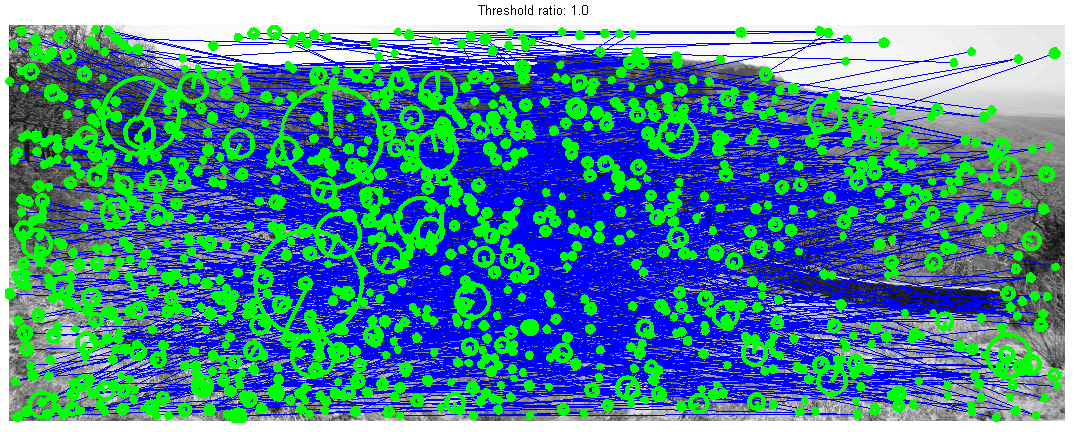
\includegraphics[width=\textwidth]{./img/ex1/matching_10_thres.png}
	\caption{Result of matching with a threshold ratio of 1.0}
	\label{fig:matching10thres}
\end{figure}

\subsection{Question 2}

{\bfseries Comment on the obtained result. Is the resulting model (more
or less) correct? By looking at the original images, do you think a linear model
is enough to model the transformation between the two images?}
